\documentclass[10pt,a4paper]{article}
\usepackage[utf8]{inputenc}
\usepackage{amsmath}
\usepackage{amsfonts}
\usepackage{amssymb}
\usepackage{tikz}
\usetikzlibrary{datavisualization}
\usetikzlibrary{datavisualization.formats.functions}
\usepackage[left=25mm,right=25mm]{geometry}
\usepackage{pgfplots}
\usepgfplotslibrary{external} 
\tikzexternalize
\usepackage{float} 
\usepackage{multicol}
\usepackage{hyperref}
\usepackage{caption}
\usepackage{subcaption}
\usepackage{csvsimple}
\graphicspath{ {./figures/} }

\begin{document}
\begin{multicols}{2}
\newenvironment{indentPar}[1]%
 {\begin{list}{}%
         {\setlength{\leftmargin}{#1}}%
         \item[]%
 }
 {\end{list}}

\begin{flushleft}
\begin{LARGE}EE 535 Lab 2: Optical Measurements of Thin Films
\end{LARGE}
\\Jonathan Hess
\\\href{https://github.com/Jetsama/EE535/tree/main/Lab2}{https://github.com/Jetsama/EE535/tree/main/Lab2}
\end{flushleft}


\section*{Abstract}

The precise thickness of a thin absorbing wafer can be found using the transmission observed from a spectrophotometer. This procedure was done for amorphous silicon (aSi) and zinc selenide (ZnSe) wafers with unknown widths.





\section*{Introduction}

Two wafers of different materials were observed with a spectrophotometer to yield measurements of The method evaluated in this paper to calculate the wafer film's width uses the transmition measured as well as the peaks and valleys of the resulting graph. This is known as the Swanepoel method of calculating thin film thickness.



\section*{Definitions}
Transmission (T) is the amount of light and electromagnetic radiation that passes through a media.\\
Reflection (R) is the amount of light and electromagnetic radiation that changes direction. \\
Absorbance (A) is the measure of how much light is absorbed by a substance at a particular wavelength.\\
Reflective Index (n) is the measure of how much light slows and bends as it travels through a material when compared against the speed of light in a vacuum.
Substrate Reflective Index (s) is the measure of how much light bends as it travels through the material that the film was deposited on.
	
\section*{Experimental}
During this lab measurements of two wafers were taken. These included reflection, transmission, absorbance, refractive index, as well as instrument error. One wafer was amorphous silicon and the other was of zinc selenide (ZnSe). What was not given or know was the thickness of these wafers. These measurements were done with the Cary 5000. This spectrophotometer has a range of 175-3300nm \cite{carry} and allows for the comparison of two samples at the same time. This was used to compare the sample wafer and a blank glass simultaneously. This allows to remove influence of the glass on the wafer's measurements.\\
The medium in the spectrophotometer is air so there will be an assumption that the refraction index will be exactly 1. There will also be an assumption that the wafer's thickness is uniform. This is because the graph in figure \ref{AmSiTran} reflects a uniform thickness\cite{paper}. Because of the use of the Swanepoel method the substrate's refractive index was measured and used to calculate the absolute refractive index of the wafer. 





	

\section*{Theory}

Interference-free transmission can be calculated with using following equations.

\begin{equation}
\label{eq:trans}
T_s = \dfrac{(1-R)^2}{1-R^2}
\end{equation}

\begin{equation}
\label{eq:reflStandard}
R = ((n_1-n_2)/(n_1+n_2))^2
\end{equation}

The equation \ref{eq:reflStandard} is that standard reflection coefficient for light striking a boundary between two different mediums. Where $n_1$ is the refraction index of first media and $n_2$ is the refraction index of the second media. Because the lab uses air as a medium this will be set to 1. Also because the equation is squared the order of these two refraction indices does matter. This derives equation \ref{eq:refl} where $s =$ the refraction index of the wafer.

\begin{equation}
\label{eq:refl}
R = ((s-1)/(s+1))^2
\end{equation}

Replacing R in equation \ref{eq:trans} with equation \ref{eq:refl} yields equation \ref{eq:3}.
\begin{equation}
\label{eq:3}
T_s = ((s-1)/(s+1))^2
\end{equation}
Solving for $s$ gives refraction index in terms of transmission in equation \ref{eq:s}.
\begin{equation}
\label{eq:s}
s = \frac{1}{T_s} + (\frac{1}{T_s^2}  - 1)^{1/2}
\end{equation}
The equation for calculating interference fringe is
\begin{equation}\label{eq:interfringe}
2nd = m \lambda
\end{equation}
where m represents the integer for maximas and half integer for minima and $\lambda$.
\begin{equation}
\label{eq:TransReg}
T = \dfrac{Ax}{(B-Cx cos(\phi) )+Dx^2)}
\end{equation}

\begin{subequations}\label{eq:TransReg}
    \begin{align}
	A= 16n^2s \label{eq:A}\\
	B = (n+1)^3(n+s^2) \label{eq:B}\\
	C = 2(n^2-1)(n^2-s^2) \label{eq:C}\\
	D = (n-1)^3(n-s^2) \label{eq:D}\\
	\phi = \frac{\pi n d}{ \lambda} \label{eq:phi}\\
	x = exp(-\alpha d) \label{eq:x}
    \end{align}
\end{subequations}

Where $\lambda =$ wavelength, $x =$ absorbance, $d =$ width,  $s =$ substrate refractive index, and $n =$ complex refractive index\\
This equation is a simplification of the optical system equation where the extinction coefficient, k, has been set to 0. This is valid over most of the spectrum\cite{marq}. At the wavelengths tested silicon has a small k constant. This can be seem in figure \ref{Sik} where the value of the extinction coefficient rests at less than 0.05 during the measurement wavelengths.
\begin{figure}[H]
\label{Sik}
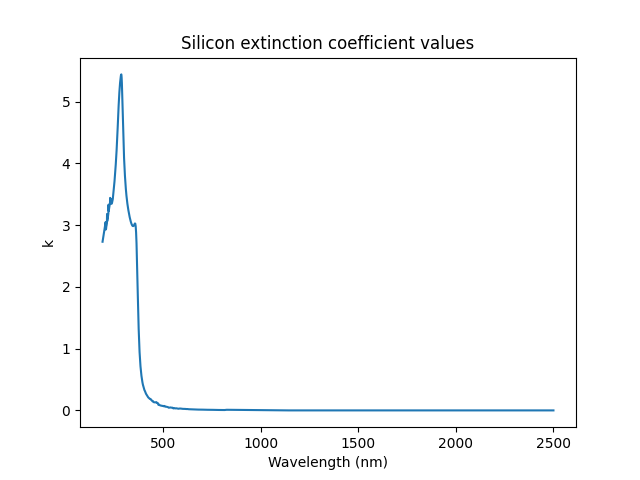
\includegraphics[scale=0.5]{Sik}
\caption{Graph showing wavelength (nm) versus the extinction coefficient of silicon\cite{siK}}
\end{figure}

The local maxima and minima are defined by the \ref{eq:TM} and \ref{eq:Tm} equations. Where $T_M$ is the local maximums and $T_m$ is the local minimums.
These equations were derived from finding where $cos(\phi) = 1$ (where the T would be at a relative max) for the maximums and  $cos(\phi) = -1$ for minimums. We can then replace $cos(\phi)$ from the with the +1 and -1 to gain the $T_M$ and $T_m$ equations\cite{marq}.
\begin{equation}
\label{eq:TM}
T_M = \dfrac{Ax}{(B-Cx)+Dx^2)}
\end{equation}

\begin{equation}
\label{eq:Tm}
T_m = \dfrac{Ax}{(B+Cx)+Dx^2)}
\end{equation}
Using these maxima (or minima) the thickness of the thin film wafer can be found 

\begin{equation}
\label{eq:d}
d = \frac{\lambda_1 \lambda_2}{2(\lambda_1 n_{e2} - \lambda_2 n_{e1})}
\end{equation}
To find the distance two extrema (either maximums or minimums) can be used along with equation \ref{eq:d}. This was done for all extrema for all 3 wafers.

\begin{equation}\label{eq:N}
N = 2s \frac{T_M -T_m}{T_M*T_m} + \frac{s^2+1}{2}
\end{equation}
\begin{equation}\label{eq:n}
n = (N + (N^2-s^2)^{1/2})^{1/2}
\end{equation}
These equations equations were derived and then used on outputted data files were using a python script which can be found in the repository.










\section*{Results}
After running the spectrometer there were data points for the two wafers. These data points included transmission, absorption and substrate reflection index.\\
The amorphous silicon wafer transmission is shown in figure \ref{AmSiTran}. This can be seen to be uniform thickness by the cosine wave imbued into the points. To use equation \ref{eq:d} extrema must be located. These were located and plotted on the graph as well as located in the table in figure \ref{AmSiTranTable}.

\begin{figure}[H]\label{AmSiTran}
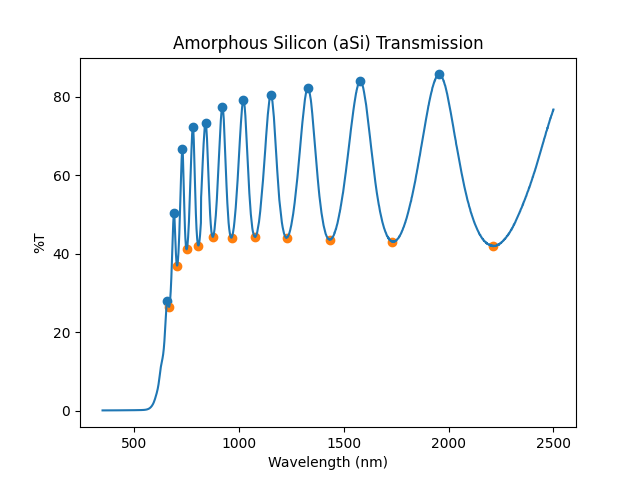
\includegraphics[scale=0.5]{AmorphousSilicon}
\caption{Graph showing wavelength (nm) versus the transmission of Wafer aSi}
\end{figure}

The local minimums and maximums were calculated using the python module scipy. The values can be seen in figure \ref{AmSiTranTable} below. Using these values combined with equation \ref{eq:TransReg} the width of the wafer.


\begin{figure}[H]
\label{AmSiTranTable}
\begin{tabular}{ |c|c|c| } 
\hline
num & maximums (nm) & minimums (nm)\\
\hline
 1 & 659  & 667\\
 2 & 691  & 705\\
 3 & 731  & 751\\
 4 & 781  & 807\\
 5 & 841  & 875\\
 6 & 921  & 965\\
 7 & 1022 & 1077\\
 8 & 1154 & 1228\\
 9 & 1328 & 1435\\
 10& 1579 & 1730\\
 11& 1954 & 2213\\
\hline
\end{tabular}
\caption{Table with wavelength of maxima and minima for the aSi wafer}
\end{figure}

Using equation \ref{eq:d} on each extrema the distance was calculated. The table and graph in figure \ref{AmSiLengthTable} show how this distance changes over region. This is because the distance should only be relied on when there is medium absorption.\\
 points 
\begin{figure}[H]\centering\label{AmSiLengthGraphwithError}

\includegraphics[scale=0.5]{asilengtherror}
\caption{Graph for wavelength of maxima and minima and calculated lengths}
\end{figure}
When analyzing the data the figures two methods were used. Originally the substrate refractive index values were calculated based on the closest refractive index to the wavelength. This created a large amount of error because the number of points was small for such a range. Instead the points were interpolated into a function. This function was then used to calculate and create the refractive index $n(\lambda)$ 

\begin{figure}[H]\centering\label{ASirefractiveindex}
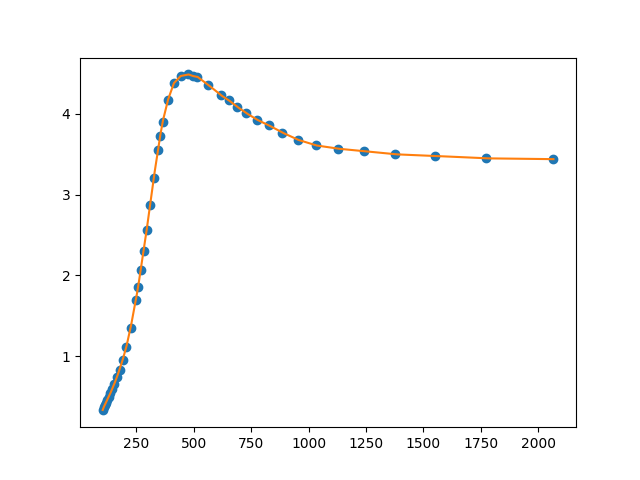
\includegraphics[scale=0.5]{ninterp}\caption{Graph for substrate interpolated refractive index}\end{figure}

\begin{figure}[H]\centering\label{AmSiLengthGraph}
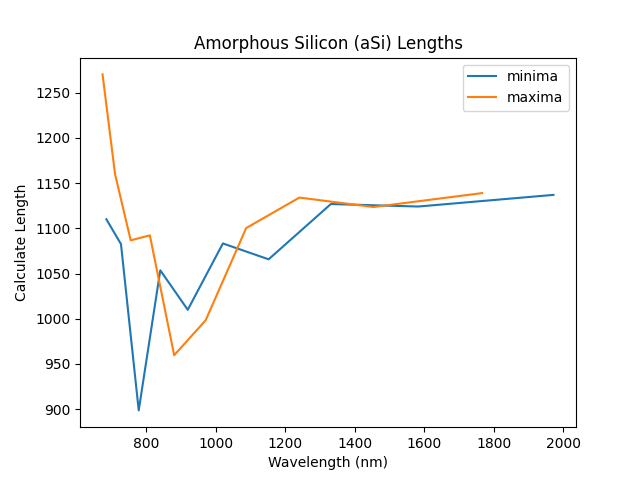
\includegraphics[scale=0.5]{asilength}
\caption{Graph for wavelength of maxima and minima and calculated lengths}
\end{figure}

\begin{figure}[H]\centering
\begin{subfigure}[b]{0.3\textwidth}\centering\label{AmSiLengthTable max}
\csvautotabular{pydata/asilengthmax.csv}
\caption{Table for wavelength of maxima and calculated lengths}
\end{subfigure}
\begin{subfigure}[b]{0.3\textwidth}\centering\label{AmSiLengthTable max}
\csvautotabular{pydata/asilengthmin.csv}
\caption{Table for wavelength of minima and calculated lengths}
\end{subfigure}
\end{figure}
There is a very large spread in width in both. This might be caused by the low number of data points of reflective index. There are 46 points across the 103.33 nm to 2066 nm range. Except after fixing this issue the range did not decrease. This is also where there was a realization that the refractive index data was actually the substrate refractive index. There is a big difference between $s$ and $n$ that was causing this massive range. After adding equation \ref{eq:n} to the python script the length distribution went down as can be seen in figure .

For better accuracy using the exact number of exterma in equation \ref{eq:interfringe}\\


The same process was done for the zinc selenide to find the thickness for that wafer. The results of the transmition is shown in figure BLL.
\begin{figure}[H]
\label{znsetran}
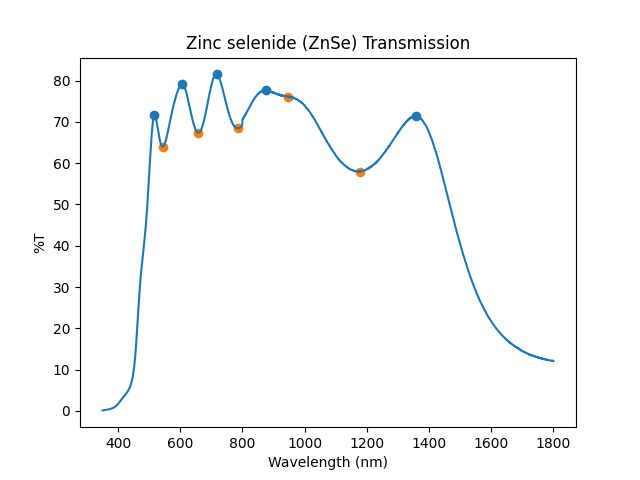
\includegraphics[scale=0.5]{znsetp}
\caption{Graph showing wavelength (nm) versus the transmission of the ZnSe Wafer }
\end{figure}
    

\section*{Appendix}
For information on the pure data or computational scripts there is a repository for this and other labs. \\
\\\href{https://github.com/Jetsama/EE535}{https://github.com/Jetsama/EE535}

\begin{thebibliography}{9}
\bibitem{book}
 Solid State Electronic Devices (2006, Prentice Hall), Ben Streetman, Sanjay Banerjee
\bibitem{Lasers}
An Entry Level Guide to Understanding Lasers (2008), Chapter 9.2.4, Jeff Hecht, 3rd ed. 

\bibitem{paper}
R Swanepoel 1983 J. Phys. E: Sci. Instrum. 16 1214

\bibitem{optical}
Optical Processes in Semiconductors, Jacques I. Pankove

\bibitem{carry}
Cary 100/300/4000/5000/6000i/7000 Spectrophotometers User's Guide

\bibitem{tauc}
How To Correctly Determine the Band Gap Energy of Modified Semiconductor Photocatalysts Based on UV–Vis Spectra, Patrycja Makuła, Michał Pacia, and Wojciech Macyk\\https://pubs.acs.org/doi/10.1021/acs.jpclett.8b02892
\bibitem{semi}
Silicon Photo Multipliers Detectors Operating in Geiger Regime: an Unlimited Device for Future Applications,Giancarlo Barbarino, Riccardo de Asmundis, Gianfranca De Rosa, Carlos Maximiliano Mollo, Stefano Russo and Daniele Vivolo


\bibitem{peaks} \href{https://erdogant.github.io/findpeaks/pages/html/Examples.html#find-peaks-in-low-sampled-dataset}{text}


\bibitem{marq} E Marquez et al 1992 J. Phys. D: Appl. Phys. 25 535
\bibitem{siK}Handbook of Optical Constants of Solids, Edward D. Palik. Academic Press, Boston, 1985 
\bibitem{GaN}Investigation of the absorption coefficient, refractive index, energy band gap, and film thickness for Al0.11Ga0.89N, Al0.03Ga0.97N, and GaN by optical transmission method
\end{thebibliography}


\end{multicols}
\end{document}
